%%% LEXICON %%%
% Block: A literal block on the workspace (like a move block)
% Chain: A series of connected blocks.
% Program: All chains on the workspace.
% Workspace: The canvas where blocks are.
% Cognitive Load: The amount of thinking needed to complete a task.
% Redundancy Effect: When redundant information causes a user to understand content less, than if the redundant content was removed
% Grammer: The structure of language that is recognized by our speech recognition
% Utterance: What is said by the user
% Recognition: What the speech recognition "hears" from the user
% Correction: The outcome of our correction algorithm on the recogition
% Toolbox: Where the available blocks can be found 

\documentclass[]{article}

\usepackage{wrapfig, algorithm, algpseudocode, amsmath, amssymb, xspace, mathalfa, graphicx}
\graphicspath{ {images/} }

% Example of this command
% \fig{MYFIGNAME001}{my caption}{size}
% See figure \ref{fig:MYFIGNAME001}

\newcommand\fig[3]{
\begin{figure}
  \begin{center}
  \includegraphics[#3]{images/#1}
  \caption{#2} 
  \label{fig:#1}
  \end{center}
\end{figure}
}

\title{Voice Programming in Computer Science Education}

\begin{document}
\maketitle

\section{Introduction}

Our goal is to create a voice enabled platform that uses machine learning to allow 
anyone to learn the fundamentals of computer science. Currently, we seek to reduce the amount
of cognitive load required to be introduced to programming concepts, which would give more 
students opportunities in computer science. 
\\ 
Voice programming looks to benefit both new and experienced programmers.  
Google Blockly is a simple language that allows us to create a robust programming grammer 
that can be used of people of all ages. In addition to discovering solutions to voice 
recognized programming, our project will help teach people who are unable to use a traditional mouse and keyboard.

\subsection{What are the results or outcome of the project?}

\section{HCI Principles}

Cognitive load,the amount of thinking requiredto complete a task, wasa main focus when
making design decisions. According to “The Limits of Speech Recognition” by Ben Shneiderman, certain
applications of speech recognition can be successful as long as the designers of the application 
focus on creating an efficient and reduced grammar. Our grammar is the structure of language that is 
recognized by our speech recognition and it is built to be as simple as possible. Simplicity for the
speech recognition aims at reducing cognitive load by reducing redundancy. In “Cognitive Load Theory”
by John Sweller, the redundancy effect is when redundant information causes a user to understand the content
less than if the redundant content was removed; therefore, using a simple grammar without redundancy,
should decrease the amount of cognitive load needed to use voice programming in computer science education.

\section{Blockly}

\subsection{What is the Blockly environment?}
Google Blockly is a JavaScript library that creates a visual block programming 
environment where core computer science logic can be taught, such as conditionals and 
looping. Blockly is run in the web browser, which gives the opportunity for mobile use. 
We chose Google Blockly over other block based languages due to its easy to work with and 
has a customizable API.

\subsection{How are blocks arranged horizontally? What language do we use to describe this?}

\subsection{How are blocks arranged vertically? What language do we use to describe this?}

\fig{workspaceDiagram.jpg}{Google Blockly workspace diagram}{width=7cm}

Blockly has a ``workspace''(See figure \ref{fig:workspaceDiagram.jpg}), which is where all of the blocks in the program are located. A ``chain of blocks''
(See figure \ref{fig:workspaceDiagram.jpg}) is used to refer to a series of connected blocks in the workspace. In Google Blockly,  
there is the ability to allow several chains of blocks to be run while
in the workspace. The order of execution causes the topmost chain of blocks. The topmost chain
is computed based off the highest vertical location of the first block in a chain. Normally, users interact
with Blockly through looking at the workspace and adding blocks to the workspace by
using a menu that holds the allowed blocks for a program, which we will refer to as the 
``toolbox'' (See figure \ref{fig:workspaceDiagram.jpg}). In order to move blocks from the toolbox to the 
workspace, usersmust click and drag using a mouse. \\

The toolbox is where available blocks can be found. Google Blockly has a large library of blocks, which can be grouped as:
\begin{itemize}
  \item$\textbf{Logic}$: if statements and equality testing
  \item$\textbf{Loops}$: while loops, for loops, for-each loops and breaking from a loop
  \item$\textbf{Math}$: incrementing variables, basic math and geometry operations, sumation and randomized numbers
  \item$\textbf{Text}$: displaying text, appending text, searching through text, substring, printing and prompting
  \item$\textbf{Lists}$: creating a list with variables, length, testing if empty and searching through a list
  \item$\textbf{Color}$: changing the color and random coloring
  \item$\textbf{Variables}$: creating a variable, setting a variable's initial value and changing a variable's value
  \item$\textbf{Functions}$: a chain of blocks with a name and possibly a return value
\end{itemize}
\section{Turtle}
Turtle, is a Blocky game, that has a ``Turtle” that can be moved the a smaller subset of commands
than what the blocky library contains. The objective of the game is to trace the path that can be found
in the Turtle canvas with the provided blocks in the toolbox. 
\textbf{Available blocks}
\begin{itemize}
  \item $\textbf{move}$: moves the tutle forward
  \item $\textbf{turn}$: turns the turtle, can decide between left or right turning and angle of turning  1,45,72,90,120,140 degrees
  \item $\textbf{repeat}$: repeats the blocks found inside, can decide to repeat either 2,3,4,5 or 360 times
  \item $\textbf{pen}$: can decide between up/down, up stops the turtle from drawing a line, down makes the turtle's movements draw lines again
\end{itemize}
Turtle is a level based system that simplifies the task of learning. By breaking the concepts of computer science into individual
levels, where each level reinforces already taught topics and introduces new topics incrementally, the amount of cognitive load
required to understand how to use each of the four blocks is greatly reduced. A natural progression of this style of teaching would be as follows:
\begin{enumerate}
  \item User is exposed to how to move the turtle forward and also turn the turtle to make a square. In order to make the square, the user
    is only give move and turn blocks, meaning they need four move blocks and three turn blocks to complete the task.
  \item User is given a repeat block in the toolbox. Now the user is tasked at completing the same task as before, but with only using one repeat
    block, one move block and one turn block.
\end{enumerate}
A user has now, in two levels, been first introduced at simply how to move and turn the turtle in the Google Blockly enviornment and then
naturally transitions into looping. Since the task is simply ``create a square'', it is not difficult to utilize the new blocks provided,
given knowledge of previous levels.
\section{Speech}

\subsection{Why did we decide to model speech using a} % This subsection heading might be incomplete?

\subsection{What choices did we make as we designed that grammar?}

\subsection{What commands are available in that grammar?}
Users must refer to blocks as the block number that is shown on the block\\
\textbf{Users can move blocks in 2 ways}:
\begin{itemize}
\item \textbf{Connect block $<$ID$>$ under block $<$ID$>$}: allows user to move blocks and chains of block under any block or chain of blocks
\item \textbf{Connect block $<$ID$>$ inside block $<$ID$>$}: allows user to move block and chains of blocks inside of a repeat block
\end{itemize}
\textbf{delete block $<$ID$>$}: deletes a block,  unless the block is the head of a chain of blocks, then this command deletes the entire chain of blocks.
\subsubsection{How does separating blocks work?}
\subsection{How do the user interface commands described earlier map to the commands in the grammar?  }

\section{Speech recognition}

\subsection{How do we perform the speech recognition? What do we use?}

\subsection{What tradeoffs are there in our decision by comparison to alternatives? What was gained and what lost?}

\clearpage

\section{Suggestions}

\subsection{Why do we give suggestions to the user? What HCI principle is behind this?}
%\subsection{What is basis on which a speech suggestion is made? What circumstances trigger it?}
%\subsection{What are the limitations of the current method and what future work might improve upon it?}
%\subsection{Show an example of the suggestions box and workspace before and after an operation}

% TODO Why do we have a suggestions list? (Well, because of the fixed grammar.
% The user is not given any training in the grammar per se.) -- done

% TODO Point out that the user might get the impression that we are giving
% suggestsions to solve the problem while we are only giving hints on how to use
% the grammar. -- done

% TODO Fix "novel algorithm", reference alg -- done
% TODO May want to shorten Alg 1 vars and describe it in text -- done
% TODO Fix quotes -- done
% TODO Why? What's the problem with always correcting? If the user says
% something utterly unrelated, we still correct it! -- done

% TODO Cite Arpabet

We provide the user a list of suggestions to teach them the grammar. We do this because the grammar is a rigid, fixed grammar. Furthermore, we provide these suggestions because we don't give any training in the grammar to the user. Instead, we hope that they can pick it up by following the suggestions. The suggestions mechanism provides generic suggestions, not specific to the block IDs or the workspace. We do not suggest how the user should solve the program, as the user might mistakenly believe. Instead, we simply teach them how to use the grammar. However, the appearance of particular suggestions is triggered by certain states of the workspace. For example, when an empty repeat block is on the canvas, we suggest that the user ``Connect block 2 inside block 1'' with these exact block IDs, regardless of what the block ID of the repeat block is. Finally, we provide an example in Table \ref{SuggestionsBeforeAndAfter} of the suggestions box with the corresponding workspace before and after adding the first block. We modify the suggestions list when we believe it could be useful for the user. For example, when there is a repeat block on the canvas, we suggest that the user connects a block inside of the repeat block, to make use of the repeat block. However, our current suggestions system is quite limited.\\
\begin{table}
	\caption{Example of suggestions before and after adding the first block to the workspace.}
	\label{SuggestionsBeforeAndAfter}
	\begin{tabular}{cccc}
		\hline
		when & workspace & suggestions \\\hline
		\\
		before & 
\includegraphics{suggestions_before_workspace.jpg} & 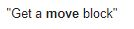
\includegraphics{suggestions_before.jpg} \\\hline
		\\
		after & 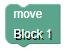
\includegraphics{suggestions_after_workspace.jpg} & 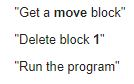
\includegraphics{suggestions_after.jpg} \\\hline
	\end{tabular}
\end{table}

\subsection{What is basis on which a speech suggestion is made? What circumstances trigger it?}

\subsection{What are the limitations of the current method and what future work might improve upon it?}

\subsection{Show an example of the suggestions box and workspace before and after an operation}

\section{Corrections}
%\textit{Utterance:} A single command given by the programmer\\
%\textit{Recognition:} What the speech reognition software recogizes an utterance as\\
%\textit{Correction:} The proposed utterance given a recognition, calculated using correction algorithm\\

%\subsection{Give an example of a common recognition error that falls out of the grammar}
%\subsection{What algorithm was used to correct recognition?}
%\subsection{If there are any parameters to be fit in this correction algorithm, how were they fit?}
As previously described, we use the Google speech API built into Google Chrome to capture user commands. However, the API has a hard time understanding commands from our grammar. We hypothesize that the API expects ordinary English, and as a result, phrases like ``get a turn block'' or ``change 4 in block 3 to 5'' are often recognized incorrectly by webkitspeechcrecognition. We developed Algorithm \ref{CorrectionAlgorithm} to correct incorrectly recognized phrases (``recognitions'') to what we hope are the intended commands (``utterances''). First, we convert the recognition into a phoneme sequence using CMU's pronouncing dictionary. Then we generate all of the possible commands that a user can specify given the workspace. We convert all of these commands into phoneme sequences and find the command whose corresponding phoneme sequence has the minimum edit distance to the recognition's phoneme sequence (breaking ties arbitrarily) and return that command. 

Furthermore, if the minimum edit-distance command is too far from the original recognition, we reject the correction and simply notify the user that we didn't understand their command. We added this feature to avoid using a ``correction'' from a completely unrelated sentence picked-up or recognized by the speech API. Our notion of ``too far'' is more concretely defined by a maximum modification factor which defines the the number of phoneme edits that can be made as a percentage of the number of phonemes in the recognition. As such, there is no fixed maximum number of edits, as this could give different performance for different string lengths. 
\begin{algorithm}
	\caption{Correction Algorithm}\label{CorrectionAlgorithm}
	\begin{algorithmic}[1]
		\Procedure{Correct}{recognition, workspace}
		\State $rphon \leftarrow stringToPhoneme(recognition)$
		\State $commands\leftarrow generatePossibleCommands(workspace) $
		\State $minEditDist \leftarrow \infty$
		\State $minEditCommand \leftarrow recognition$
		\For{$command$ in $commands$}
			\State $cphon \leftarrow stringToPhoneme(command)$
			\State $editDist \leftarrow findMinEditDist(rphon, cphon)$
			\If{$editDist < minEditDist$}
				\State $minEditCommand \leftarrow command$
				\State $minEditDist \leftarrow editDist$
			\EndIf
		\EndFor
		\If{$minEditDist <= maxModification * length(rphon)$}
			\State \Return{$minEditCommand$}
		\Else
			\State \Return{$recognition$}
		\EndIf
		\State \Return{$minEditCommand$}
		\EndProcedure
	\end{algorithmic}
\end{algorithm}

We determined the threshold in the following way.

\subsection{If there are any parameters to be fit in this correction algorithm, how were they fit?}
\subsubsection{What statistical procedure was use?}
\subsubsection{What data was gathered?}
\subsubsection{What assumptions were made that could be considered weaknesses of the model?}
\subsection{Give an example of a common case that the corrections algorithm, as currently implemented, fails on}

\section{Layout}

%\subsection{How are commands interpreted visually?}
%\subsection{Where do new blocks go?}
%\subsection{How are blocks reordered when one is moved?}
%\subsection{What happens if the user runs out of space on the workspace?}
%\subsection{Describe the layout algorithm in pseudocode}
%\subsection{Show an example of the a before and after with the layout algorithm}
%\subsection{Are there any cases that currently give problems for the layout algorithm?}

As the user writes a program, certain locations on the workspace fill with blocks.
This presents a challenge: what should happen when blocks overlap with one another?
For our system to be practically useful, it must avoid introducing such visual impairments,
which may prevent the user from issuing commands (e.g. if they cannot see a block ID)
or which may introduce unnecessary cognitive load.

Blockly by default places new blocks at the top left of the workspace, even if the new block
will overlap an old block. Similarly, when Blockly connects one block to another, the resulting chain
might overlap another chain.

We devise simple layout algorithms for each case. To make this formal, we view
the workspace as a 2D plane $W$ where the origin is the top left corner, the $x$ axis ranges from 0
to $\textsc{Width}(W)$, and the $y$ axis ranges from 0 to $\textsc{Height}(W)$.
Let $B$ denote the set of blocks on the workspace and let $m$ denote a small, constant margin.
In our implementation, we choose $m = 20$ (pixels) because it is small enough to preserve space
on the workspace, and large enough to prevent Blockly from automatically connecting nearby blocks.

\textbf{Adding Blocks} We place new blocks by finding the vertically lowest free
position on the workspace and placing the new block there, exactky $m$ pixels right of
the flyout. This is summarized by Algorithm~\ref{alg:place}.

\textbf{Moving Blocks} Suppose the user has just connected one block to another, and the
resulting chain now overlaps $n$ blocks. We repair the layout by moving the $n$ conflicting
blocks individually via Algorithm~\ref{alg:relayout}. 

\begin{algorithm}[H]
\caption{Place New Block}\label{alg:place}
\begin{algorithmic}
\Procedure{PlaceNewBlock}{$B, m$}
\State $\ell \gets m$ \Comment{stores lowest $y$ on the workspace}
\For{$b \in B$} 
	\If{$y_b + h_b \ge \ell$}
		\State $\ell \gets y_b + h_b + m$
	\EndIf
\EndFor
\State \Return $(m, \ell)$
\EndProcedure
\end{algorithmic}
\end{algorithm}

\begin{algorithm}[H]
\caption{Relayout Existing Block}\label{alg:relayout}
\begin{algorithmic}
\Procedure{Relayout}{$b, B, W, m$}
\State $x \gets m$
\While{$x < \textsc{width}(W)$}
	\State $y \gets m$
	\While{$y < \textsc{height}(W)$}
		\If{$\textsc{EphemeralMove}(b, (x,y))$ and no conflicts} 
				\State $\textsc{Move}(b, (x,y))$
		\EndIf
		\State $y \gets y + m$
	\EndWhile
	\State $x \gets x + m$
\EndWhile
\State $\textsc{Move}(b, (m,m))$
\EndProcedure
\end{algorithmic}
\end{algorithm}

\section{Related Work}

\subsection{What is the related work in speech interfaces for programming?}

\subsection{What is the related work in speech interfaces for computer science education?}


\section{Future Work}

\end{document}
